\subsection*{Independence}

\begin{definition}[Independence]
    Two events $A$ and $B$ are \emph{independent} if:
    \[
        P(A|B) = P(A) \quad \text{or} \quad P(B|A) = P(B)
    \]
\end{definition}

\begin{corollary}[Product Rule for Independent Events]
    If $A$ and $B$ are independent, then:
    \[
        P(A \cap B) = P(A) \cdot P(B)
    \]
    This follows immediately from probability rule (R4.1)[cite: 2].
\end{corollary}

\begin{theorem}[Independence of Complements]
    If $A$ and $B$ are independent, then their complements $A'$ and $B'$ are also independent[cite: 2].
\end{theorem}

\begin{proofbox}
    Using De Morgan's Law and probability rules:
    \begin{align*}
        P(A' \cap B') &= P((A \cup B)') \\[1ex]
        &= 1 - P(A \cup B) \\[1ex]
        &= 1 - P(A) - P(B) + P(A \cap B) \\[1ex]
        &= 1 - P(A) - P(B) + P(A) \cdot P(B) \quad \text{(by independence)} \\[1ex]
        &= (1 - P(A)) \cdot 1 - (1 - P(A)) \cdot P(B) \\[1ex]
        &= (1 - P(A))(1 - P(B)) \\[1ex]
        &= P(A') \cdot P(B')
    \end{align*}
\end{proofbox}

\begin{example}[Dependence in semiconductor manufacturing]
    Consider the semiconductor manufacturing scenario from the previous learning task:
    \[
        \left.
        \begin{aligned}
            P(B) &= 0.024 \\
            P(B|A) &= 0.10
        \end{aligned}
        \right\} \implies A \text{ and } B \text{ are dependent events.}
    \]
\end{example}

\begin{example}[Reliability of a three-device circuit]
    Given a circuit with three components $A$, $B$, and $C$, assume that the individual devices function independently.
    Let $P(A) = 0.95$, $P(B) = 0.95$, and $P(C) = 0.90$ denote the operational probabilities.

    \begin{center}
        \begin{tikzpicture}[>=stealth]
            \def\shift{2/3}
            \foreach \label/\x/\y in {A/0/1, B/0/-1, C/2/0}
            {
                \node[device] (device\label) at (\x, \y) {$\label$};
            }

            \coordinate (topleft) at ($(deviceA.west)+(-\shift,0)$);
            \coordinate (topright) at ($(deviceA.east)+(\shift,0)$);
            \coordinate (bottomleft) at ($(deviceB.west)+(-\shift,0)$);
            \coordinate (bottomright) at ($(deviceB.east)+(\shift,0)$);

            \coordinate (leftAB) at ($(topleft)!.5!(bottomleft)$);
            \coordinate (rightAB) at ($(topright)!.5!(bottomright)$);

            \draw (deviceA) -- (topleft) -- (bottomleft) -- (deviceB);
            \draw (deviceA) -- (topright) -- (bottomright) -- (deviceB);

            \draw (leftAB) -- ++(-2*\shift,0);
            \draw (rightAB) -- (deviceC);
            \draw (deviceC) -- ++(2*\shift,0);
        \end{tikzpicture}
        \captionof{figure}{Circuit diagram with three independent devices.}
        \label{fig:2.5}
    \end{center}\medskip

    Let the individual operational probabilities be given as $P(A) = 0.95$, $P(B) = 0.95$, and $P(C) = 0.90$.
    The overall probability that the circuit functions is formulated as:
    \[
    P(\text{circuit functions}) = P((A \cup B) \cap C) = P(A \cup B) \cdot P(C)
    \]

    To compute the parallel subsystem reliability $P(A \cup B)$:
    \begin{align*}
        P(A \cup B) &= P(A) + P(B) - P(A \cap B) \\
        &= P(A) + P(B) - P(A) \cdot P(B) \\
        &= 0.95 + 0.95 - (0.95)^2 \\
        &= 0.9975
    \end{align*}
    Thus, the operational probability is:
    \[
        P(\text{circuit functions}) = 0.9975 \cdot 0.90 = \mathbf{0.89775} \quad (\approx 0.8978)
    \]
\end{example}   

\paragraph{Alternative method for parallel components}
An alternative approach to evaluating the parallel subsystem $A \cup B$ uses complement probabilities:
\begin{align*}
    P(A \cup B) &= 1 - P((A \cup B)') \\
    &= 1 - P(A' \cap B') \\
    &= 1 - P(A') \cdot P(B') \quad \text{(by independence)} \\
    &= 1 - (1 - P(A))(1 - P(B)) \\
    &= 1 - (0.05)^2 = 0.9975
\end{align*}
So $P(\text{circuit functions}) = 0.9975 \cdot 0.9 = \mathbf{0.89775}$.


\subsection*{Bayes' Theorem}

We revisit once again the semiconductor example from the previous learning task.
Suppose a semiconductor fails ($B$).
To find the probability that the chip was subjected to high contamination levels during manufacturing ($A$),
we evaluate the inverse conditional probability $P(A|B)$.

When evaluating conditional probabilities in reverse operational order, Bayes' Theorem is applied.

\begin{theorem}[Bayes' Theorem]
    For two events $A$ and $B$ with $P(B) > 0$, it holds that:
    \[
        P(A|B) = \frac{P(B|A) \cdot P(A)}{P(B)}.
    \]
\end{theorem}
\begin{proofbox}[Bayes' Theorem]
    From rules (R4.1) and (R4.2), we can express $P(A \cap B)$ both as $P(B|A)\cdot P(A)$ and $P(A|B) \cdot P(B)$. 
    Dividing both expressions by $P(B)$ (which is allowed, as $P(B)$ is not zero) yields:
    \[
        P(A|B) = \frac{P(A \cap B)}{P(B)} = \frac{P(B|A) \cdot P(A)}{P(B)}
    \]
\end{proofbox}

\begin{center}
    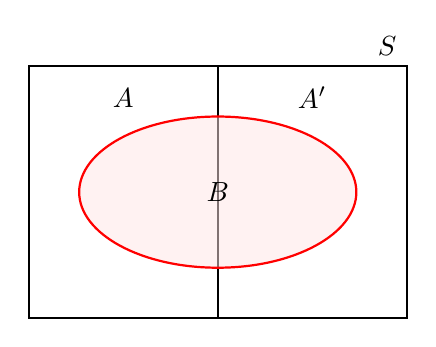
\begin{tikzpicture}[scale=0.8]
        \draw[thick] (0,0) rectangle (6,4) node[above left] {$S$};
        \draw[thick] (3,0) -- (3,4);
        \node at (1.5,3.5) {$A$};
        \node at (4.5,3.5) {$A'$};
        \draw[red, thick, fill=red!10, fill opacity=0.5] (3,2) ellipse (2.2 and 1.2) node[opacity=1, color=black] {$B$};
    \end{tikzpicture}
    \captionof{figure}{Partitioning of event $B$ across sample space partitions $A$ and $A'$.}
    \label{fig:bayes-theorem-partition}
\end{center}

By definition of conditional probability and the Law of Total Probability:
\[
    P(A|B) = \frac{P(A \cap B)}{P(B)} = \frac{P(B|A)P(A)}{P(B)}
\]

\begin{example}[Semiconductor manufacturing]
    Revisiting the semiconductor example, we calculate $P(\text{high contamination} \mid \text{semiconductor fails}) = P(A|B)$:
    \[
        P(A|B) = \frac{P(B|A) \cdot P(A)}{P(B|A) \cdot P(A) + P(B|A') \cdot P(A')} = \frac{0.10 \cdot 0.20}{0.024} = \frac{0.02}{0.024} \approx \mathbf{0.8333}
    \]
\end{example}

\subsection*{Random Variables}

Given a random experiment $E$ with associated sample space $S$ (for instance, engaging a target in up to five attempts, $S = \set{h, mh, mmh, mmmh, mmmmh}$ where $m = \text{miss}$ and $h = \text{hit}$):

\begin{definition}[Random Variable]
    A function $X$ that assigns a real number to each outcome in the sample space $S$ is called a \emph{random variable}.
    \begin{itemize}\setlength\itemsep{0.5em}
        \item A \textbf{discrete random variable} is a random variable with a finite or countably infinite range.
        \item A \textbf{continuous random variable} has a range consisting of an interval (either finite or infinite) of real numbers.
    \end{itemize}
\end{definition}

\begin{example}[target engagement]
    In engaging a target up to five attempts, let $X$ represent the attempt number on which the target is eliminated.
    Here, $X(mmh) = 3$ and $X(h) = 1$.
    Because the range of $X$ is the finite set $\set{1, 2, 3, 4, 5}$, $X$ is a discrete random variable.
\end{example}

\begin{example}[lifespan analysis]
    Let $X$ denote the operational lifespan of a light bulb.
    Since the range of $X = \set{x \in \mathbb{R} \mid x \ge 0}$ forms a continuous real interval, $X$ is a continuous random variable.
\end{example}

\begin{example}[keep trying until first success]
    Consider engaging a target in an infinite sequence of independent attempts with a constant single-trial success probability $p$.
    Let $X$ denote the attempt number on which the target is eliminated.
    Because the range of $X = \set{1, 2, 3, \dots}$ is countably infinite, $X$ is a discrete random variable.
\end{example}